\section{Analyse de l'existant}

\subsection {Présentation générale}
Actuellement le savoir-faire est très limité, en effet il y a peu de processus de gestion déclenchés pour surveiller les sites. Le schéma ci-dessous résume la surveillance actuelle.\\

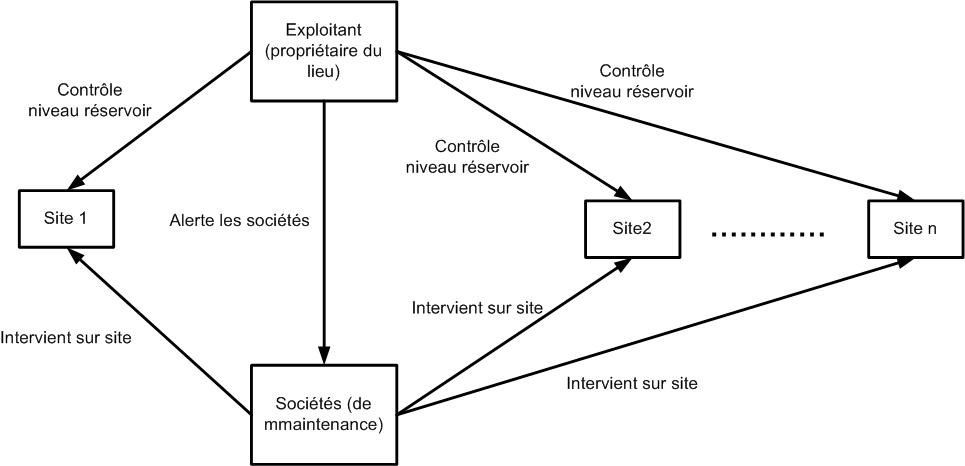
\includegraphics[width=0.9\textwidth]{img/schemaAnalyseExistant.png}

~\\
Le matériel est celui utilisé par les sociétés de maintenance intervenant sur les sites (camions, systèmes de vidage/remplissage..)
Deux métiers ont été identifiés, les propriétaires des sites s’occupent de leur exploitation tandis que les sociétés spécialisés sont chargées du métier de la maintenance.

\subsection {Contexte géographique}

COPEVUE gère actuellement de nombreux sites isolés concernés par le système à mettre en place. Ils peuvent être situés aussi bien dans les pays Nordiques de l'UE que dans certaines régions méditerrannéennes. La principale caractéristique de ces sites est leur isolement : ils sont généralement dans des régions peu peuplées et sont difficiles à atteindre. \\
Le premier déploiement de la solution proposée à cette appel d'offre s'effectuera dans la partie Nord de la Norvège.


\subsection {Fonctionnement actuel}

Le contrôle des sites isolés est actuellement effectué directement leur propriétaire. Ils doivent se rendre sur chacun de leurs sites afin d'effectuer les vérifications appropriées et appeler la société spécialisée chargée de la maintenance du site si nécessaire.\\
Nous pouvons aisément constater en observant le mode de fonctionnement actuel son manque d'efficacité, de fiabilité et d'économie de ressources. En effet, faire se déplacer les propriétaires à intervalles réguliers sur leurs sites est très coûteux en temps de trajets (certains propriétaires possèdent de nombreux sites éloignés les uns des autres). Ces déplacement engendrent un coût non négligeable en raison des distances à parcourir. \\
La fiabilité des tests est également relativement faible en raison de l'intervalle de temps entre deux mesures sur une même cuve, celle-ci pouvant nécessiter une maintenance urgente si le niveau d'une cuve atteint un seuil critique. Un contrôle, même régulier des propriétaires ne permet pas de détecter le dépassement du seuil critique dans un délai suffisamment court.\\
Enfin, lorsque les propriétaires signalement un besoin de maintenance à une entreprise spécialisée, il est impossible à l'heure actuelle, de savoir si un autre site à proximité aurait un besoin similaire. Les camions chargés de la maintenance des différents sites sont donc sous-exploités et sont contraints d'effectuer de nombreux allers-retours entre les différents sites et leur base.

\subsection {Existant informatique}

COPEVUE n'a actuellement aucune gestion informatique centrale des différents sites isolés.

\section{Concurrence}

Sur le marché européen notre société tient encore largement sa place. Cependant, des sociétés concurrentes existent et ont toujours une part importante du marché. Les principales sont : National Instruments et AllianTech.

        \subsection{Axys Technologies INC}
        AXYS Technologies Inc (AXYS) est une compagnie canadienne ayant plus de 30 ans d'expérience dans la conception, la fabrication et l'installation de systèmes de télésurveillance de l'environnement à travers le monde. AXYS applique ses connaissances approfondies dans divers domaines : celui marin, dans des stations de surveillance terrestres et offshore, dans des systèmes d'évaluation des ressources éoliennes de mesure des paramètres aquatiques, océaniques et atmosphériques. La société propose également les services techniques sur le terrain pour former et soutenir les clients dans l'exploitation et la maintenance de tous les produits. Le système embarqué que nous préconisons pour notre système est d'ailleurs fabriqué par leur compagnie. Leur système semble être le plus abouti, aujourd'hui le système embarqué qu'il fabrique est l'un des meilleurs du marché. Il propose une solution comprenant les 3 composants suivants :
\begin{description}
           \item[Watchman500 Node :] Permettant de collecter les données des capteurs
           \item[Data Management System (DMS) :] Permettant fr configurer le système embarqué.
           \item[Smart Web et Smart View :] Sont une application web et un logiciel permettant de superviser à distance le site et d'exploiter les données recueillis. Ils permettent également d'exporter les données sous divers formats (CSV, XMl, Excel..)
\end{description}

        \subsection{National Instruments}
        Il semble être l'un des leaders sur notre domaine d'activité. La société est basé à Austin au Texas, elle a été créée en 1976. Elle a ses filiales dans plus de quarante pays. Un aspect qui nous permet de les concurrencer est qu'aucune industrie ne représente plus de 10% de leurs ventes, en effet ils ont des activités très variées. Il investisse 16% de leur chiffre d'affaires annuel dans la recherche et le développement et sorte en moyenne 208 produits par an. Ce qui fait d'eux, assez souvent, un précurseur dans leurs domaines d'activités. 
        Il propose un système personnalisable appelé WSN très semblable à celui que nous mettrons en place, qui permet également la surveillance en extérieur d'équipements.



\section {Bilan de quelques dysfonctionnements}
Plusieurs dysfonctionnements ont déja été identifés : 
\begin{itemize}
	\item La non regularite des surveillances par les exploitants (proprietaires des sites)
	\item La non assurance de la maintenance directement par une societe quand elle est contactee car son parc ne dispose pas de camions disponibles.
	\item Les risques de désastres humains et environnementaux encourus.
\end{itemize}
	Le nouveau systeme devra remedier aux problemes detectees en : 
\begin{itemize}
	\item Autonome pour ne pas necessiter d'interventions humaines regulieres pour des operations de constat ou de maintenance
	\item Generique car sera implente sur differents sites
	\item Pilotable a distance (configuration, commande..)
	\item Fiable vu les enjeux environnements en jeu
\end{itemize}	
	Par rapport au systeme actuel il permettra une surveillance temps reel a partir d'un poste distant. 
	Il permettra egalement de réduire considerablement les interventions et d'avoir une meilleur planification de celles-ci, afin de réaliser des economies logistiques tout en garatissant certaines autres exigences (criticite, meilleur surveillance..).


\section{Axes d'améliorations}

Les principaux axes d'amélioration du nouveau système sont :

\begin{itemize}
\item Automatisation du système de surveillance des sites
\item Suivi temps réel des sites avec possibilité de configurations/commandes à distance
\item Amélioration de la communication (systèmes embarquées, capteurs..)
\item Diminution des coûts de transports
\item Diminution des coûts de main d'œuvre
\item Fiabilité du système de surveillance au vue de risques écologiques
\item Traçabilité des informations et opérations
\item Généricité/Facilité d'évolution du système
\end{itemize}
